\section{Energy Consumption}
\label{sec:res:energy}

In this section, we look at the energy consumption of the {\tracker} application described in \autoref{sec:impl:project:ii}.
The measurements was performed using the {\STK} and {\BIO} boards.
The {\tracker} is an interrupt driven application and has two modes of operation from an energy consumption perspective.
It turns \emph{On} for each interrupt to perform the measurement and turns \emph{Off} when the measuring is complete.

\subsection{Measuring}
The measurement was performed with the \emph{Energy Profiler} application supplied by Silicon Labs as a part of their \emph{Simplicity Studio} software suite.
The profiler measures on board current at a sample frequency of 6250Hz.
Power, measured in Watt (J/s), is given by the formula $P (J/s) = V*I $, where \emph{V} is voltage and \emph{I} is current.
By accumulating the Power over time, we get the energy consumption given in \emph{Joule}.
This metric is reported by the \emph{Energy Profiler}.

Each measurement, called a \emph{run}, was gathered manually by executing the sample collection process (see \autoref{sec:project:i:sample-collection}) for 30s and recording the energy reported by the profiler.
This process was repeated four times for each data point, and an average was calculated after removing the sample with the highest variance.
This process was introduced to remove human error from the manual collection.
The number of collected and discarded samples were based upon the stability of the results, and the largest variance in the collected samples were 0.174\%.

\subsection{Parameter}

The energy consumption was recorded for the {\tracker}, which was configured with different workloads.
The workload is dependent on how many interrupts are trigger per run, and how much work is performed during each interrupt.
To vary the workload, the number of triggered interrupts were varied by configuring the length of the interval between each interrupt while the work was held constant for each interrupt.
\autoref{tab:res:energy:parameters} gives the interrupt interval and the corresponding number of interrupts per \emph{run} used for the measurement.

\begin{table}[H]
  \centering
  \begin{tabular}{l | c | c}
    \textbf{Interval} & \textbf{\# of Interrupts/\emph{run}} & \textbf{Execution time} \\
    \hline
    25ms & 1200 & 30s \\
    50ms & 600 & 30s \\
    100ms & 300 & 30s \\
    500ms & 60 & 30s \\
    1000ms & 30 & 30s \\
    \hline
  \end{tabular}
  \caption{Interrupt Interval Parameter}
  \label{tab:res:energy:parameters}
\end{table}

The measurement was performed at all the standard optimization levels provided by the compilers.
This was done to remove the bias where different applications have better performance using different optimization levels.
As noted in \autoref{sec:res:code-size} these are \emph{O0}, \emph{O1}, \emph{O2}, \emph{O3} and \emph{Os} (only available for {\C}).
As we will see in the results below, by including all the optimization levels, we uncovered another bias related to energy consumptions.
The \emph{O0} levels were only evaluated with debugging symbols.

\subsection{Results}

In this section, we look at the results of the energy consumption measurement.
We first look at the whole picture by presenting all the measurements produced by the set of possible parameters.
Later, we will consider the best configuration for {\C} application together with the best configured {\rust} application for each workload.

\begin{figure}[H]

  \centering
  \begin{subfigure}{0.40\textwidth}
    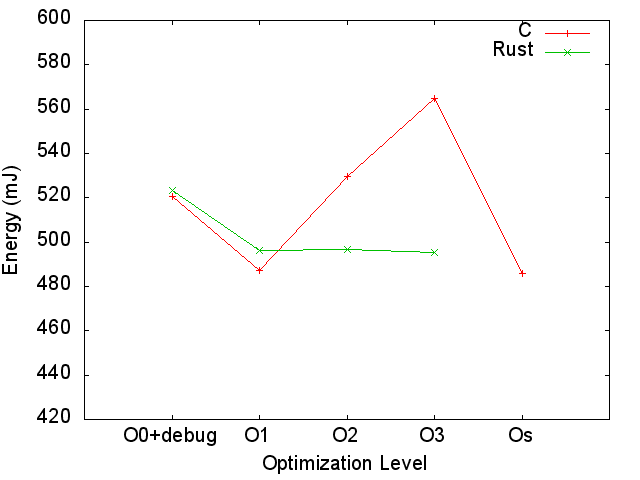
\includegraphics[width=\textwidth]{results/plots/energy/25.png}
    \caption{25ms}
  \end{subfigure}
  \hfill
  \begin{subfigure}{0.40\textwidth}
    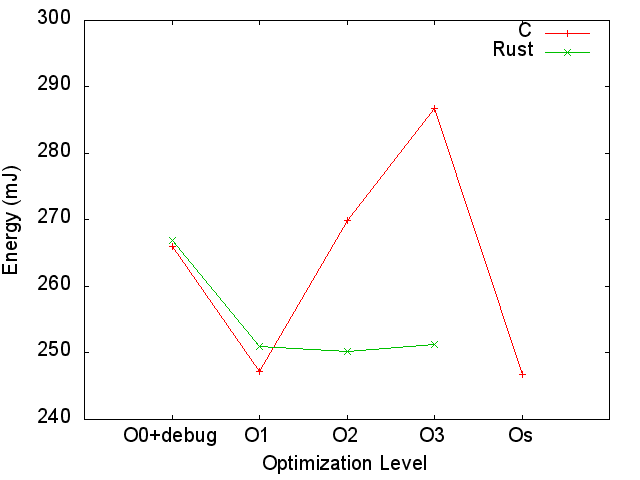
\includegraphics[width=\textwidth]{results/plots/energy/50.png}
    \caption{50ms}
  \end{subfigure}

    \begin{subfigure}{0.40\textwidth}
    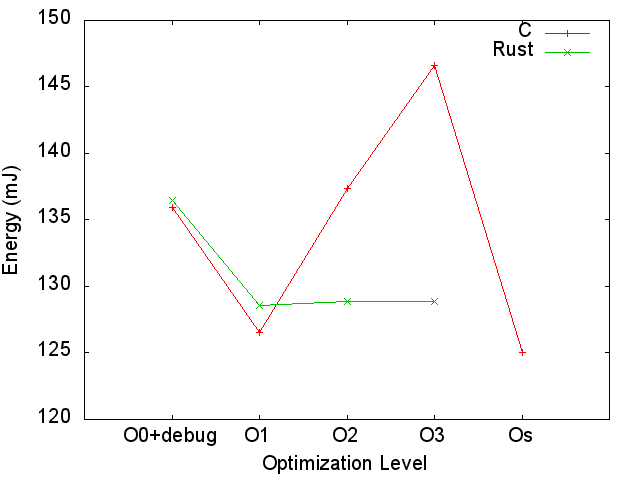
\includegraphics[width=\textwidth]{results/plots/energy/100.png}
    \caption{100ms}
  \end{subfigure}
  \hfill
  \begin{subfigure}{0.40\textwidth}
    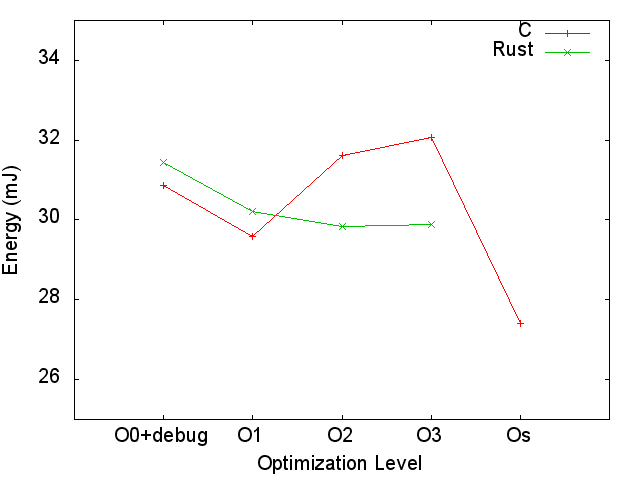
\includegraphics[width=\textwidth]{results/plots/energy/500.png}
    \caption{500ms}
  \end{subfigure}

  \begin{subfigure}{0.40\textwidth}
    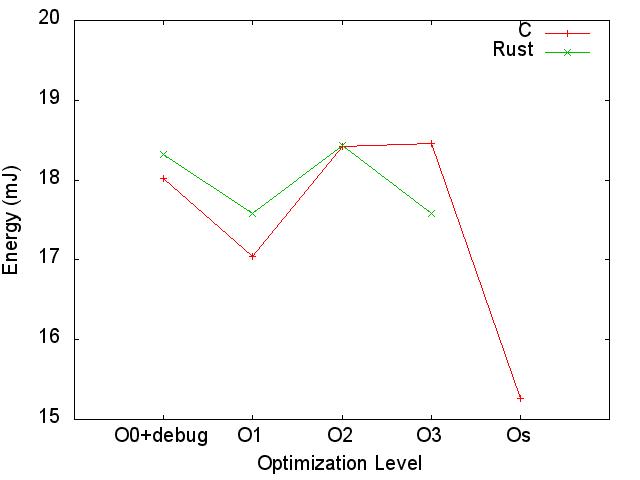
\includegraphics[width=\textwidth]{results/plots/energy/1000.png}
    \caption{1000ms}
  \end{subfigure}

  \caption{Comparison between {\rust} and {\C} for each workload}
  \label{fig:res:energy:comparison}
\end{figure}

\autoref{fig:res:energy:comparison} shows the energy consumption for each of the workloads and compares the optimization levels for {\rust} and {\C}.
We see that {\rust} and {\C} have comparable consumption in each of the workload configurations.
It is also evident that an external bias, investigated below, accounts for the variance between the various optimization levels.

Now we look at the relative performance comparing the version with lowest energy consumption for each workload.
For the {\C} code, we can easily see from \autoref{fig:res:energy:comparison} that this is produced by the \emph{Os} level.
The {\rust} versions, on the other hand, are either \emph{O1}, \emph{O2} or \emph{O3}, although the difference is never larger that 1\%.

\begin{figure}[H]
  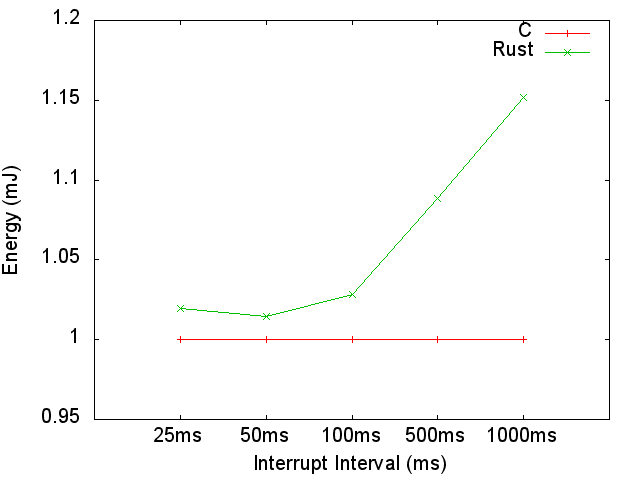
\includegraphics[width=\textwidth]{results/plots/energy/best.png}
  \caption{{\rust} vs {\C} relative comparisons for best builds}
  \label{fig:res:energy:best}
\end{figure}

\autoref{fig:res:energy:best} shows the relative energy consumption by setting the consumption of the {\C} \emph{Os} build to 1 for each of the workload.
The {\rust} line plots the best performing {\rust} builds relative to this {\C} build.
For reference, the results for the \emph{O3} optimization level of the {\C} build is included.
We see that the {\rust} code always performs within $\sim$15\% of the {\C} code and is always better than the \emph{O3} line.


The variance between the different optimization levels of {\C} code in \autoref{fig:res:energy:comparison} was unexpected.
In this application, we anticipated that higher optimization levels would result in faster interrupt handlers and thus lower energy consumption.
When the initial results did not meet this expectation, we used the \emph{Energy Profiler} to plot the instantaneous current drawn by the application.

\begin{figure}[H]
  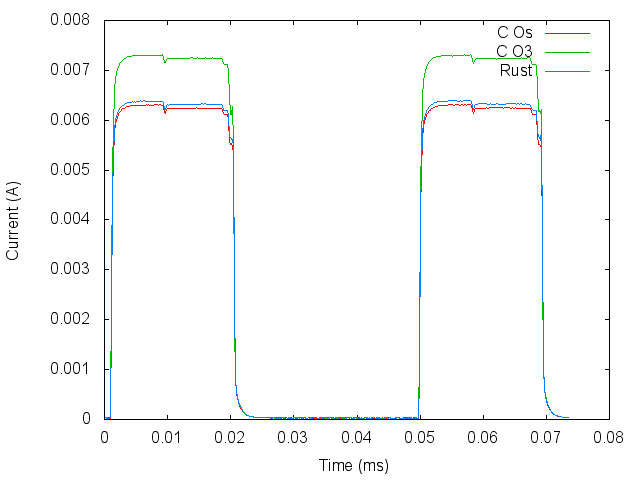
\includegraphics[width=\textwidth]{results/plots/energy/irq/50.png}
  \caption{Current of 50ms workload}
  \label{fig:res:energy:current}
\end{figure}

\autoref{fig:res:energy:current} plots the current drawn by the {\gecko} while handling an interrupt and the idle state between interrupts.
The first thing to notice about the plot is that the time it takes to handle an interrupt is constant for the various optimization levels.
The second point is the difference in current drawn by the {\gecko} while handling the interrupts.
We can see the O3 level draws more current compared to the Os level; we found the reason for this when we looked at the instruction cache hit ratio.

\begin{table}[H]
  \centering
  \begin{tabular}{l | l | l | l | l}
    \textbf{Language} & \textbf{Level} & \textbf{Hits} & \textbf{Misses} & \textbf{Hit Ratio} \\
    \hline
    C & O3 & 110969 & 43429 & 71.9\% \\
    C & Os & 162029 & 614 & 99.6\% \\
    \hline
  \end{tabular}
  \caption{Cache hit ratio for optimized {\C} binaries}
  \label{tab:res:energy:cache}
\end{table}

\autoref{tab:res:energy:cache} shows the cache hit ratios recorded for binaries presented in \autoref{fig:res:energy:current}.
We see that the cache hit ratio for the binary compiled with O3 has a hit ratio of $\sim$72\% while the Os level has as high as $\sim$99\%.
The lower instruction cache hit ratio causes the {\gecko} to load instructions from flash more frequently and thus consumes more energy.
This effect was not studied any closer, but can possibly be explained by the O3 level producing code which is to large for the instruction cache to contain.
